\documentclass[12pt, letterpaper]{article}
\usepackage[utf8]{inputenc}
\usepackage{graphicx}
\usepackage[T1]{fontenc}
\graphicspath{ {/} }



\title{Malloc and free ID1206 Operating Systems}
\author{Frida Johansson}
\date{December 2021}

\begin{document}

\maketitle
\section{First implementation}
For the first run I implemented a benchmark program for a BUFFER size of 100 running for 1000 rounds.
To achieve a sequence of non-identical requests a random index was calculated in each loop and then accessed the BUFFER of that particular index.
If it was NULL, \textbf{dalloc()} was called, else \textbf{dfree()} was called. 


\subsection{First run}

Before the \textbf{merge()} function was implemented a few benchmarks was done. To bench the length of the freelist, different ranges of the requested size value was tested.
The list became longer when smaller blocks was used and shorter when larger blocks were used. Since more smaller blocks could fit the freelist rather than larger ones it affected 
the length and thus ended up in more headers.
It is very unefficient to have so many headers that takes so much unnecessary space, and even more so when the headers are 24 bytes.
Since we havn't implemented \textbf{merge()} yet we will have to accept a 24 byte header for each and every block. The average block size of the freelist was 188 bytes when 
the interval of the size requests was between 8 and 500. When MAX was set to 5000 and increased the interval it was 489 bytes. It became larger, as expected, but still the average 
block size in freelist is not as big as we might want to and there are many headers that takes a lot of space.

\begin{figure}[h]
    \center
    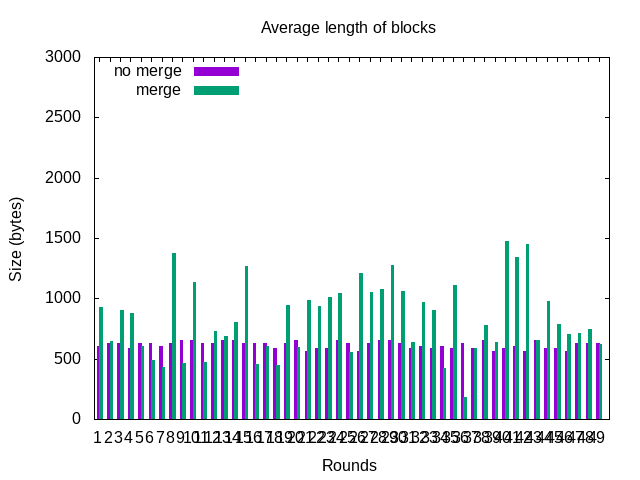
\includegraphics[scale=0.65]{graph0.png}
    \caption{Average size block, selected randomly between 8 and 5000 bytes}
    \label{fig:graph0}
\end{figure}

However, when \textbf{merge()} is implemented things are getting a bit better. \textbf{merge()} is checking if previous and next blocks are free. 
If they are free it will merge them to one large block with one header. Figure 1 shows the different average size of the blocks depending if \textbf{merge()} is implemented or 
not. Your could see that when \textbf{merge()} is implemented, the blocks are in general larger. For example, if we would have two free blocks, with a 24 byte header each, 
those would instead become one large block with one 24 byte header. The other 24 byte header wouldn't be needed anymore and instead be free space. 
The length of the freelist becomes shorter as there are not as many small blocks as before and thus not so many headers. By implementing \textbf{merge()} we can 
avoid a lot of unnecessary headers that takes a lot of space that basically just says that the next block is free as well. If \textbf{merge()} isn't implemented, we wouldn't
be able to accomodate requests for larger blocks since we would probably just have a bunch of headers pointing to small areas of free space.
For example, if we had two free blocks of 32 bytes each and want to request for 64 bytes the system would let us know that it doesn't exists - when it in fact does. 
By implementing \textbf{merge()} we can accomodate those requests since blocks next to each other are merged and we will skip extra unnecessary headers. 
When freeing up all space, all 65488 bytes was freed when implementing \textbf{merge()}. This was not the case when \textbf{merge()} wasn't implemented since headers of size 24 bytes each was still left.
See Figure 2 below for the freelist length when merge is implemented and not.
\begin{figure}[h]
    \center
    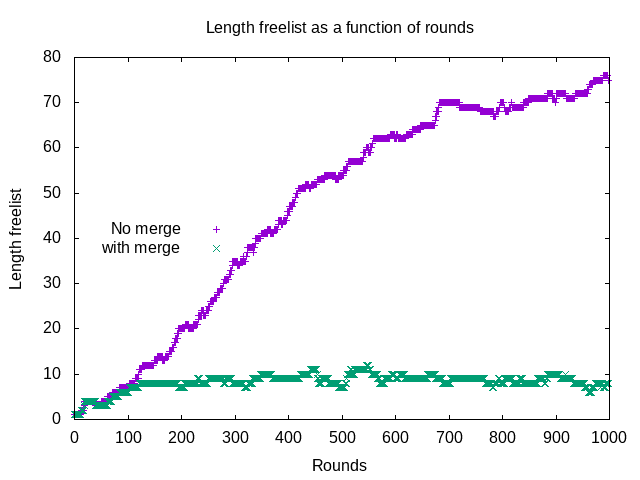
\includegraphics[scale=0.65]{graph1.png}
    \caption{Difference in length of freelist between merge and no merge}
    \label{fig:graph1}
\end{figure}

\section{Improving performance -Size of head}

By reducing the size of the header it doesn't only save us memory, but it goes faster when accessing and writing to it as well.
By looking at the graph in Figure 3 that becomes quite obvious. To clarify this we can look at the \textbf{head} structure and the \textbf{taken} structure.
The \textbf{head} has a total of 24 bytes header. Together with 16 bytes allocation it results in 40 bytes. The \textbf{taken} structure has a total of 8 bytes header.
Together with 16 bytes allocation it results in 24 bytes in total. When running the program with the \textbf{head} a total of 40 bytes must be fetched.
Instead of fetching 40 bytes, we can then use the \textbf{taken} structure as header and fetch 24 bytes instead. By choosing \textbf{taken} we could fit more
blocks in the caches since 24 bytes is less than 40 bytes. The chance to get a cache hit increases and also the chance to get a cache hit again thanks to spatial locality. 
At some points the improved header \textbf{taken} takes longer time, but a reason for that could be when a cache miss occurs.

\begin{figure}[h]
    \center
    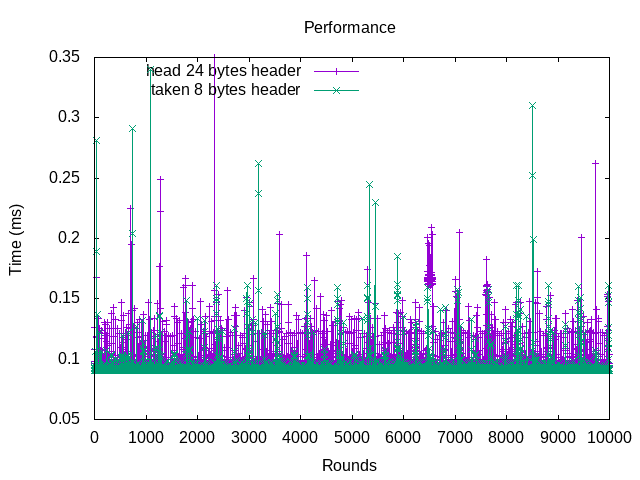
\includegraphics[scale=0.65]{graph2.png}
    \caption{Performance difference between different size of header}
    \label{fig:graph2}
\end{figure}

\section{Discusson - "To be free or not to be, dfree is the question"}

I struggled a while with the \textbf{split()} function. At first I thought the function was suppose to return the freelist block, and not the block we allocated. 
So, when that function returned to \textbf{find()} I putted the returned block with the requested size back in the freelist and returned the block that had the calculated 
remaining size of the freelist to the user. This ended up very badly but when I structured everything up, drew pictures and printed out what was actually happening I saw that 
it was wrong. I could then adjust my code and put the block with the remaining size of the freelist back in the freelist and return the block we allocated with its correct size.

The ending of this report will be about a problem every programmer face. Typos. I sat a whole day with the GDB debugger and tried to figure out what was wrong since
I could only run my code with a specific size of the buffer and a specific size of ROUNDS. If the buffer was 100 I could go for 100 runs, not more. If I wanted to increase 
my rounds I also had to increase the size of my buffer. The problem was obviously in dfree but I couldn't see where I could possible done wrong since everything seemed to be 
fine and was suppose to be working. The GDB debugger didn't return the exact line where the actual problem was, it just returned where it simply didn't work anymore and returned 
\emph{Segmentation fault}. At last I saw that the problem was in \textbf{dfree()} function where I accidently written \emph{aft->free = TRUE;} instead of \emph{aft->bfree = TRUE;}.

\end{document}

